\documentclass[a4paper,10pt]{article}
%\documentclass[a4paper,10pt]{report} for proposal
\usepackage[T1]{fontenc}
\usepackage[latin9]{inputenc}
%\usepackage[utf8]{inputenc}
%\usepackage{graphicx}
%\usepackage{epstopdf}
\usepackage{array}
\usepackage{times}
 \usepackage[pdftex]{hyperref}
%\usepackage[pdftex]{graphicx}
%\usepackage[dvips]{graphicx}
\usepackage{graphicx,epstopdf}
\epstopdfsetup{suffix=}
\DeclareGraphicsExtensions{.ps}
\DeclareGraphicsRule{.ps}{pdf}{.pdf}{`ps2pdf -dEPSCrop -dNOSAFER #1 \noexpand\OutputFile}
\usepackage{float}
\usepackage{amsfonts}
\usepackage[affil-it]{authblk}
\usepackage{amsthm}
\usepackage{amsmath}
\usepackage{amssymb}
\usepackage{color}
\usepackage{tikz}
\usepackage{subcaption}
\usepackage[export]{adjustbox}
\usepackage{wrapfig}
\usepackage{multirow}
\textwidth 16.5truecm \textheight 20truecm \hoffset -2.2truecm
\numberwithin{equation}{section}
%\usepackage[backend=bibtex,
%style=numeric,
%bibencoding=ascii,
%%style=alphabetic
%%style=reading
%sorting=ynt
%]{biblatex}
\usepackage[english]{babel}
\usepackage[nottoc]{tocbibind}
\usepackage[numbers,sort]{natbib}
\usepackage{textcomp,gensymb}
\bibliographystyle{abbrvnat}



%\addbibresource{review.bib}
\title{Supplement Information}

\author{Yining Lu}
\affil{Department of Mathematics,\\University of Michigan}


\date{}
\begin{document}

\maketitle

%\tableofcontents

\section{Mathematical Model}

A model consisting several indispensable  reactions to produce oscillations is presented in Eq.\ref{eq:minimum}. 
\begin{equation}
\begin{gathered}
\mathrm U \overset{k_{\mathrm{a}}}{\underset{+\mathrm {KaiA}}{\longrightarrow}} \mathrm U^{*}\\
\mathrm U \overset{k_{\mathrm {b}}}{\longleftarrow} \mathrm U^{*} \overset{ k_\mathrm f}{\longrightarrow} \mathrm T \overset{ k_\mathrm{ps}}{\longrightarrow} \mathrm{ST} \\
\mathrm {ST}+\mathrm B\overset{ k_{2}^{\mathrm{on}}}{\underset{k_{2}^{\mathrm{off}}}{\rightleftarrows}} \mathrm {B\cdot ST} \\
\mathrm {B\cdot ST} \overset{ k_{\mathrm{dps}}}{\longrightarrow} \mathrm{B\cdot S} \quad
\mathrm {B\cdot S} \overset{ k_{\mathrm{dps}}}{\longrightarrow} \mathrm{B\cdot U} \quad
\mathrm U+\mathrm B\overset{ k_{1}^{\mathrm{on}}}{\underset{k_{1}^{\mathrm{off}}}{\rightleftarrows}} \mathrm {B\cdot U}
\end{gathered}\label{eq:minimum}
\end{equation}
Adding some reactions in Eq.\ref{eq:minimum} leads to an alternative model Eq.\ref{eq:full} following the same design rules. We argue that different alternations on the original simple model in \ref{eq:minimum} does not affect the validity of important results including temperature compensation, which is discussed in detail in a later section.
\begin{equation}
\begin{gathered}
\mathrm U \overset{k_{\mathrm{a}}}{\underset{+\mathrm {KaiA}}{\longrightarrow}} \mathrm U^{*}, \quad \mathrm U \overset{k_{\mathrm {b}}}{\longleftarrow} \mathrm U^{*} \overset{ k_\mathrm {cat}}{\longrightarrow} \mathrm T 
\\ 
\mathrm T \overset{k_{\mathrm{a}}}{\underset{+\mathrm {KaiA}}{\longrightarrow}} \mathrm T^{*},\quad \mathrm T \overset{k_{\mathrm {b}}}{\longleftarrow} \mathrm T^{*} \overset{ k_\mathrm{cat}}{\longrightarrow} \mathrm{ST} \\
\mathrm{U} \overset{ k_\mathrm{ps}}{\longrightarrow} \mathrm{T} \overset{ k_\mathrm{ps}}{\longrightarrow} \mathrm{ST} \\
\mathrm {ST}+\mathrm B\overset{ k_{2}^{\mathrm{on}}}{\underset{k_{2}^{\mathrm{off}}}{\rightleftarrows}} \mathrm {B\cdot ST},\quad \mathrm S+\mathrm B\overset{ k_{3}^{\mathrm{on}}}{\underset{k_{3}^{\mathrm{off}}}{\rightleftarrows}} \mathrm {B\cdot S},\quad \mathrm U+\mathrm B\overset{ k_{1}^{\mathrm{on}}}{\underset{k_{1}^{\mathrm{off}}}{\rightleftarrows}} \mathrm {B\cdot U}\\
\mathrm {B\cdot ST} \overset{ k_{\mathrm{dps}}}{\longrightarrow} \mathrm{B\cdot S}, \quad
\mathrm {B\cdot S} \overset{ k_{\mathrm{dps}}}{\longrightarrow} \mathrm{B\cdot U}\\
 \mathrm{ST} \overset{ k_\mathrm{dps}}{\longrightarrow} \mathrm{S} \overset{ k_\mathrm{dps}}{\longrightarrow} \mathrm{U} \\
\end{gathered}\label{eq:full}
\end{equation}

First model assumes that there are multiple phosphorylation levels of KaiC with differentiated phosphorylation process in each step. Unphosphorylated KaiC binds with KaiA with high affinity and enters an unstable phosphorylation state (KaiC-P$^{*}$), this catalytic process is quick enough that we can assume equilibrium. Another way to understand is that almost immediately after the phosphorylation step, the enzyme KaiA drops off from KaiC. 
Unstable KaiC-P$^{*}$ can then slowly stabilize by either falling back to be unphosphorylated or proceeding forward into a stable phosphorylated state KaiC-P$_{1}$. Once proceeded into a stable phosphorylation state, KaiC-P$_{1}$ go through a few more slow phosphorylation steps. Finally a highly phosphorylated KaiC protein can bind with KaiB into KaiB$\cdot$KaiC complex which sequester KaiA activity by eliminating the free KaiA in a linear fashion. KaiB$\cdot$KaiC complex can then dephosphorylate while still sequestering KaiA. Here we also argue that unlike the complicated phosphorylation phase, KaiC dephosphorylation can proceed in one step at a slow rate. Finally, KaiB falls off the unphosphorylated KaiB$\cdot$KaiC complex, thus freeing more KaiA protein to catalyze the first phosphorylation step and start over another oscillation cycle. 

% The key reactions in this first model are listed below where we denote by U the unphosphorylated KaiC, P$^{*}$ the unstable phosphorylated state and P$_{i}$'s ($i=1,2,3,4$) the stable phosphorylated KaiC states, along with KaiBC complexes represented in a natural way:

% \begin{gather*}
% \mathrm U \overset{k_{\mathrm{a}}}{\underset{+\mathrm {KaiA}}{\longrightarrow}} \mathrm P^{*}\\
% \mathrm U \overset{k_{\mathrm {b}}}{\longleftarrow} \mathrm P^{*} \overset{ k_\mathrm f}{\longrightarrow} \mathrm P_1 \overset{ k_\mathrm{ps}}{\longrightarrow} \mathrm{P_2} \overset{ k_\mathrm{ps}}{\longrightarrow} \mathrm{P_3} \overset{ k_\mathrm{ps}}{\longrightarrow} \mathrm{P_4}\\
% \mathrm P_4+\mathrm B\overset{ k_{2}^{\mathrm{on}}}{\underset{k_{2}^{\mathrm{off}}}{\rightleftarrows}} \mathrm {P_4\cdot B} \\
% \mathrm {P_4\cdot B} \overset{ k_{\mathrm{dps}}}{\longrightarrow} \mathrm{U\cdot B} \\
% \mathrm U+\mathrm B\overset{ k_{1}^{\mathrm{on}}}{\underset{k_{1}^{\mathrm{off}}}{\rightleftarrows}} \mathrm {U\cdot B}
% \end{gather*}
                                                                                               
The corresponding mass action equations are as follows:
\begin{align*}
\frac{d[U]}{dt}&=k_{\mathrm b}[P^{*}]-k_{\mathrm{a}} [A][U]+k_{1}^{\mathrm{off}}[UB] -k_{1}^{\mathrm{on}}[U][B] \\
\frac{d[P^{*}]}{dt}&=k_{\mathrm{ps}} [A][U]-(k_{\mathrm f}+k_{\mathrm b})[P^{*}]\\
\frac{d[P_{1}]}{dt}&=k_{\mathrm f}[P^{*}]-k_{\mathrm{ps}}[P_{1}]\\
\frac{d[P_{i}]}{dt}&=k_{\mathrm{ps}}([P_{i-1}]-[P_{i}]) \quad \mathrm{for} \quad i=2,3\\
\frac{d[P_{4}]}{dt}&=k_{\mathrm{ps}}[P_{3}]+k_{2}^{\mathrm{off}}[BP_{4}] -k_{2}^{\mathrm{on}}[P_{4}][B] \\
\frac{d[P_{4}B]}{dt}&=-k_{\mathrm{dps}}[P_{4}B]-k_{2}^{\mathrm{off}}[P_{4}B] +k_{2}^{\mathrm{on}}[P_{4}][B]\\
\frac{d[UB]}{dt}&=k_{\mathrm{dps}}[P_{4}B]-k_{1}^{\mathrm{off}}[UB] +k_{1}^{\mathrm{on}}[U][B]
\end{align*}

%We also assume that complex P$_{4}$B and UB can both sequester KaiA through tight binding and KaiA unbinds only when KaiB falls off the complex. 

%The sequestration of KaiA is modeled in the following way such that the amount of free KaiA negatively depend on KaiBC complex concentration [UB] and [P$_{4}$B]. Here we choose the strength of binding sequestration of both complexes to be 2, but the choice of strength factor doesn't change the nature of our model. One can also verify that the sequestration scheme is quite robust in the sense that whether [UB] sequesters KaiA or not doesn't affect the qualitative feature. More detailed discussion of whether all the KaiBC complex need to sequester KaiA and whether the choice of sequestration strength affects the oscillation will be in a later section.
\begin{align*}
[B]&=[B]_{T}-[UB]-[P_{4}B]\\
[A]&=\max\{0,[A]_{T}-n\cdot \left([UB]+[P_{4}B]\right) \}\quad n=2
\end{align*}

%Simulating the model we can obtain good oscillations for a wide range of reaction rates parameters. 



\section{Linear Stability Analysis}
Here we present mathematical analysis of the simplified model including a linear stability analysis and a limiting procedure. 
We continue to use $[T], [ST], [S]$ as the state variables for KaiC concentrations and $[A]$ the concentration of KaiA. Constants $C_T$ and $A_T$ indicate the total amount of the KaiC and KaiA proteins respectively and $K_d$ is the dissociation constant in the sequestration of KaiA through KaiC-S. We assume that the sequestration happens on a faster timescale, thus reaching equilibrium quickly. Due to the different time scale and the fact that the binding of KaiA doesn't impact other reactions of $S$, we can solve for the concentration of free KaiA.

\begin{gather*}
[A][S_{\mathrm{free}}]=K_d[AS]\\
\implies (A_T-[AS])([S]-[AS])=K_d[AS]\\
\implies 
[AS]=\left(A_T+[S]+K_d-\sqrt{(A_T+[S]+K_d)^2-4A_T[S]}\right)/2\\
\implies 
[A]=A_T-[AS]=\left(A_T-[S]-K_d+\sqrt{(A_T-[S]-K_d)^2+4K_dA_T}\right)/2
\end{gather*}


The system of equations describing our simple mechanism can therefore be written as follows.  Here we reduce the number of variables by applying the conservation law $[U]=C_T-[T]-[ST]-[S]$.  



\begin{align*}
\frac{\mathrm{d}[T]}{\mathrm{d}t}&=k_1 [A] (C_T-\mathrm{[T]}-\mathrm{[ST]}-\mathrm{[S]})-k_2 \mathrm{[T]}\\
\frac{\mathrm{d}[ST]}{\mathrm{d}t}&=k_2 [T]-k_3 [ST]\\
\frac{\mathrm{d}[S]}{\mathrm{d}t}&=k_3 [ST]-k_4 [S]\\
[A]&=\left(A_T-[S]-K_d+\sqrt{(A_T-[S]-K_d)^2+4K_dA_T}\right)/2
\end{align*}
Our simulation shows that $K_d$ has to be small enough for the system to oscillate. Therefore when $K_d\ll A_T$, we can take limit as $K_d\to 0$ in $[A]$ to get an approximated expression $[A]=\max\{ A_T-[S],0 \}$.
The system is then simplified to:
\begin{align}
\frac{\mathrm{d}[T]}{\mathrm{d}t}&=k_1 (A_T-[S]) (C_T-\mathrm{[T]}-\mathrm{[ST]}-\mathrm{[S]})-k_2 \mathrm{[T]}\label{eq:dt}\\
\frac{\mathrm{d}[ST]}{\mathrm{d}t}&=k_2 [T]-k_3 [ST]\label{eq:dst}\\
\frac{\mathrm{d}[S]}{\mathrm{d}t}&=k_3 [ST]-k_4 [S]\label{eq:ds}
\end{align}

Solving the system for the equilibrium solutions, we obtain $[ST]=\frac{k_4}{k_3} [S],[T]=\frac{k_4}{k_2}  [S]$ from Eq.(\ref{eq:dst}) and Eq. (\ref{eq:ds}). With all other variables plugged in, Eq.(\ref{eq:dt}) can be reduced to a quadratic in terms of $[S]$.
\[k_1(A_T-[S])(C_T-(1+\frac{k_4}{k_2}+\frac{k_4}{k_3})[S])-k_4[S]=0\] 
In addition, we assume $k_4\ll k_1$ since KaiA-enhanced phosphorylation is much faster then (auto)phosphorylation. Hence we can drop the last term $k_4[S]$ in the quadratic equation by dividing $k_1$ through all terms and find two steady state solutions:
\begin{gather*}
(A_T-[S])(C_T-(1+\frac{k_4}{k_2}+\frac{k_4}{k_3})[S])-\frac{k_4}{k_1}[S]=0\\
\implies
(A_T-[S])(C_T-(\frac{k_4}{k_2}+\frac{k_4}{k_3})[S])=0\\
\implies [S]^*=A_T, \quad [S]^*=\frac{C_T}{1+r}, \quad \mathrm{where}\quad r=\frac{k_4}{k_2}+\frac{k_4}{k_3}
\end{gather*}


First, we compute the Jacobian at the second equilibrium $[S]^*=A_T$
\begin{equation}\label{eq:jacobian1}
J_1=
\begin{pmatrix}
-k_2 & 0 & -k_1(C_T-(1+r)A_T)\\
k_2 & -k_3 & 0\\
0 & k_3 & -k_4 
\end{pmatrix}
\end{equation}
The corresponding characteristic function is then:
\[f_2(\lambda)=(\lambda+k_2)(\lambda+k_3)(\lambda+k_4)+k_1k_2k_3(C_T-(1+r)A_T)\]
We conclude from the secant condition that oscillations occur when 
\begin{gather*}
\frac{k_1k_2k_3(C_T-(1+r)A_T)}{k_2k_3k_4}\geq (\sec (\frac{\pi}{3}))^3
\end{gather*}
\begin{equation}\label{eq:ctatcondition}
C_T-(1+r)A_T\geq \frac{8k_4}{k_1}
\end{equation}
To verify our analysis, we simulate the model when $k_2=k_3=k_4=0.1$ and compare our results with $C_T-3A_T>\frac{0.8}{k_4}$. 

In order to analyze the Jacobian matrix at the second equilibrium without introducing too much computational details, we further assume that $k_2=k_3=k_4$ which means the autodephosphorylation and the autphosphorylation of KaiC are on the same time scale.
The Jacobian  $[S]^*=\frac{C_T}{3}$  can be then simplified

\begin{equation}\label{eq:jacobian2}
J_2=
\begin{pmatrix}
-k_1(A_T-\frac{C_T}{3})-k_2 & -k_1(A_T-\frac{C_T}{3}) & -k_1(A_T-\frac{C_T}{3})\\
k_2 & -k_2 & 0\\
0 & k_2 & -k_2 
\end{pmatrix}
\end{equation}
The characteristic function of \ref{eq:jacobian2} is a cubic function:
\begin{equation}
\begin{split}
f_2(\lambda)&=(b+k_2+\lambda)(k_2+\lambda)^2+bk_2(k_2+\lambda)+bk_2^2\\
&=(\lambda+k_2)^3+b(k_2+\lambda)^2+bk_2(k_2+\lambda)+bk_2^2\\
&=\lambda^3+(3k_2+b)\lambda^2+(3k_2^2+3bk_2)\lambda+k_2^3+3bk_2^2
\end{split}
\end{equation}
where $b=k_1(A_T-\frac{C_T}{3})>0$.

The Routh-Hurwitz Stability Criterion tells us that a necessary condition for a cubic function $h(x)=x^3+a_2x^2+a_1x+a_0$ to be stable (all of its roots have negative real part) is $a_0>0, a_2>0, a_2a_1>a_0$.

Applying this to our cubic function above, we already have $a_0>0,a_2>0$ and we compute the third one accordingly:
\begin{equation}
\begin{split}
a_1a_2-a_0&=(3k_2+b)(3k_2^2+3bk_2)-k_2^3+3bk_2^2\\&
=(3k_2+b)(3k_2+3b)-k_2^2+3bk_2\\&
=8k_2^2+9bk_2+3b^2\\
&>0 \qquad \qquad \forall\; b,k_2>0
\end{split}
\end{equation}
Therefore we know that all three roots of the characteristic function always have nagative roots, meaning the steady state is stable and there is no oscillations around that point.



\section{Reproducing experimental results}

Notice that the choice of parameter set does not change any quantitative results. Our model is simulated with different initial conditions to produce dynamics under different situations when it is incubated with KaiA only (Fig\ref{fig:A+C}), KaiB only  (Fig \ref{fig:B+C}) and alone (Fig \ref{fig:conly}). 

Existing experimental results from \citet{kitayama2003} suggest that KaiB alone does not affect the (de)phosphorylation process of KaiC. Indeed we observe from our simulations that the profile of KaiC doesn't change much when KaiB is added into the system. Without KaiA, adding KaiB to KaiC produces the same phosphorylation profile (see Fig.\ref{fig:B+C} and Fig.\ref{fig:conly}).

\begin{figure}[H]
\centering
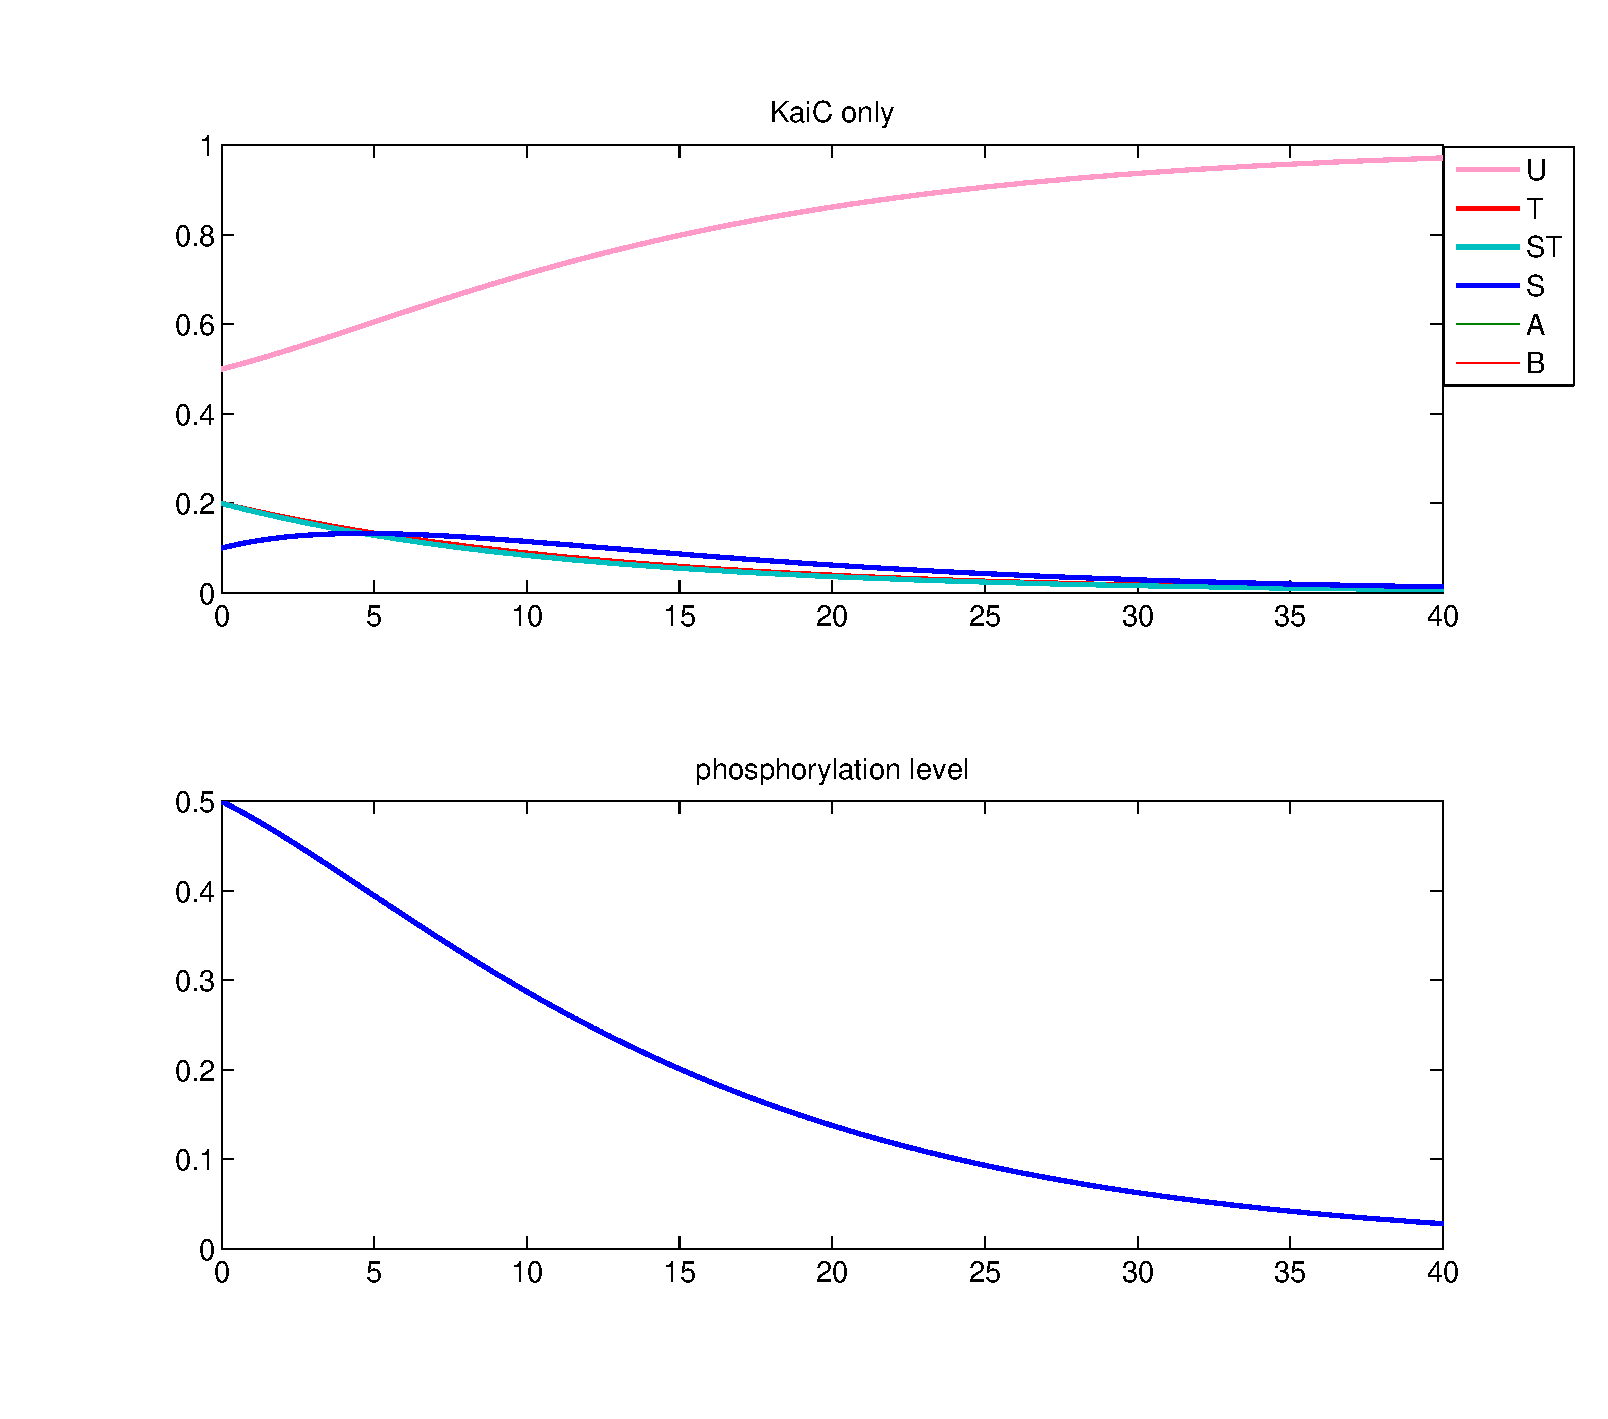
\includegraphics[scale=0.6]{Conly.eps}
\caption{\fontfamily{lmss}\selectfont Temporal profiles of different KaiC complexes as well as the overall phosphorylation level without any KaiA or KaiB in the system. Initially KaiC is 50\% phosphorylated. Complexes that remain zero concentration due to initial conditions are omitted in the graph.}
\label{fig:conly}
\end{figure}

\begin{figure}
\centering
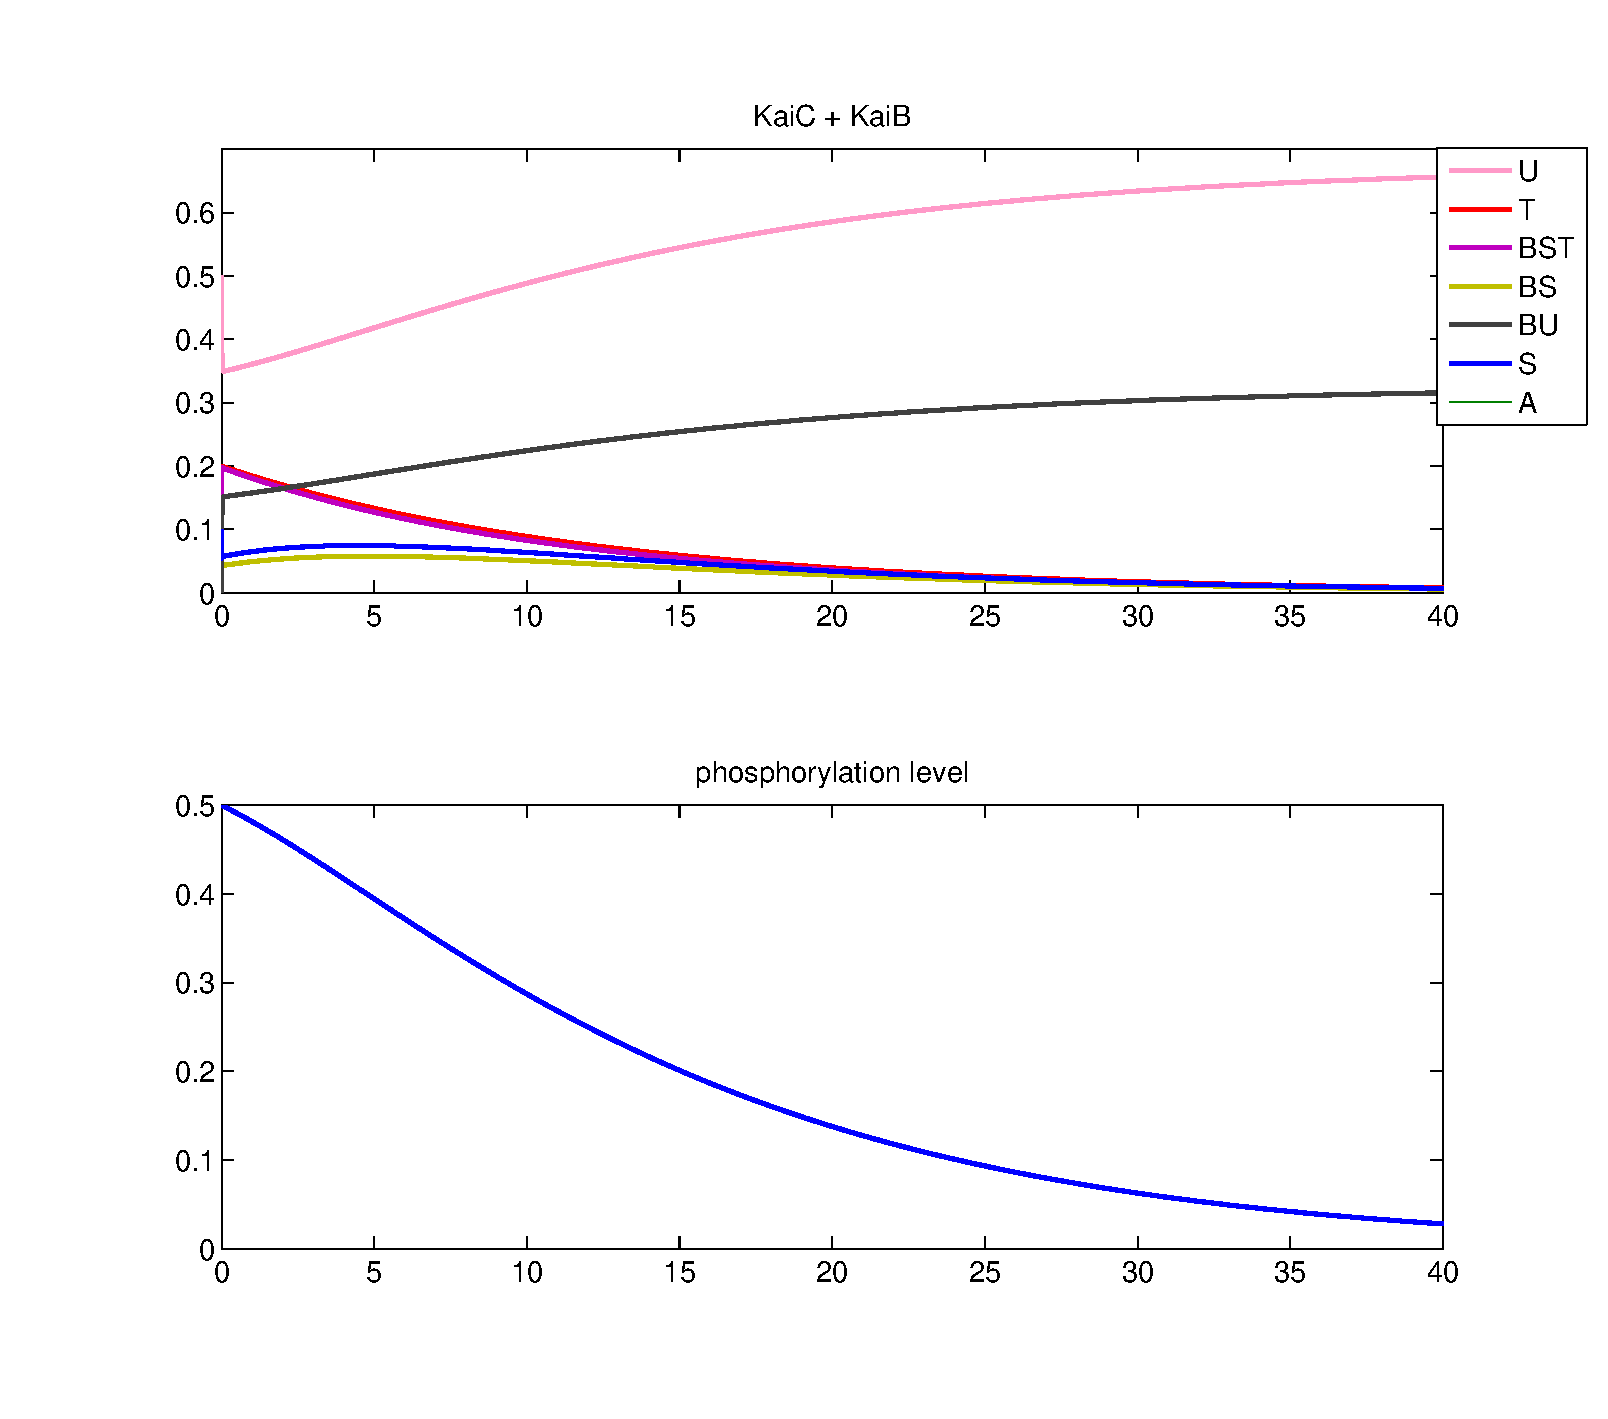
\includegraphics[scale=0.6]{B+C.eps}
\caption{\fontfamily{lmss}\selectfont Temporal profiles of different KaiC complexes as well as the overall phosphorylation level without any KaiA in the system. Initially KaiC is 50\% phosphorylated. Complexes that remain zero concentration due to initial conditions are omitted in the graph.}
\label{fig:B+C}
\end{figure}
It is also observed that when incubated with KaiA alone, the KaiC proteins will be driven to a highly phosphorylated state, consistent with results from \citet{Tamito2005}.
\begin{figure}[H]
\centering
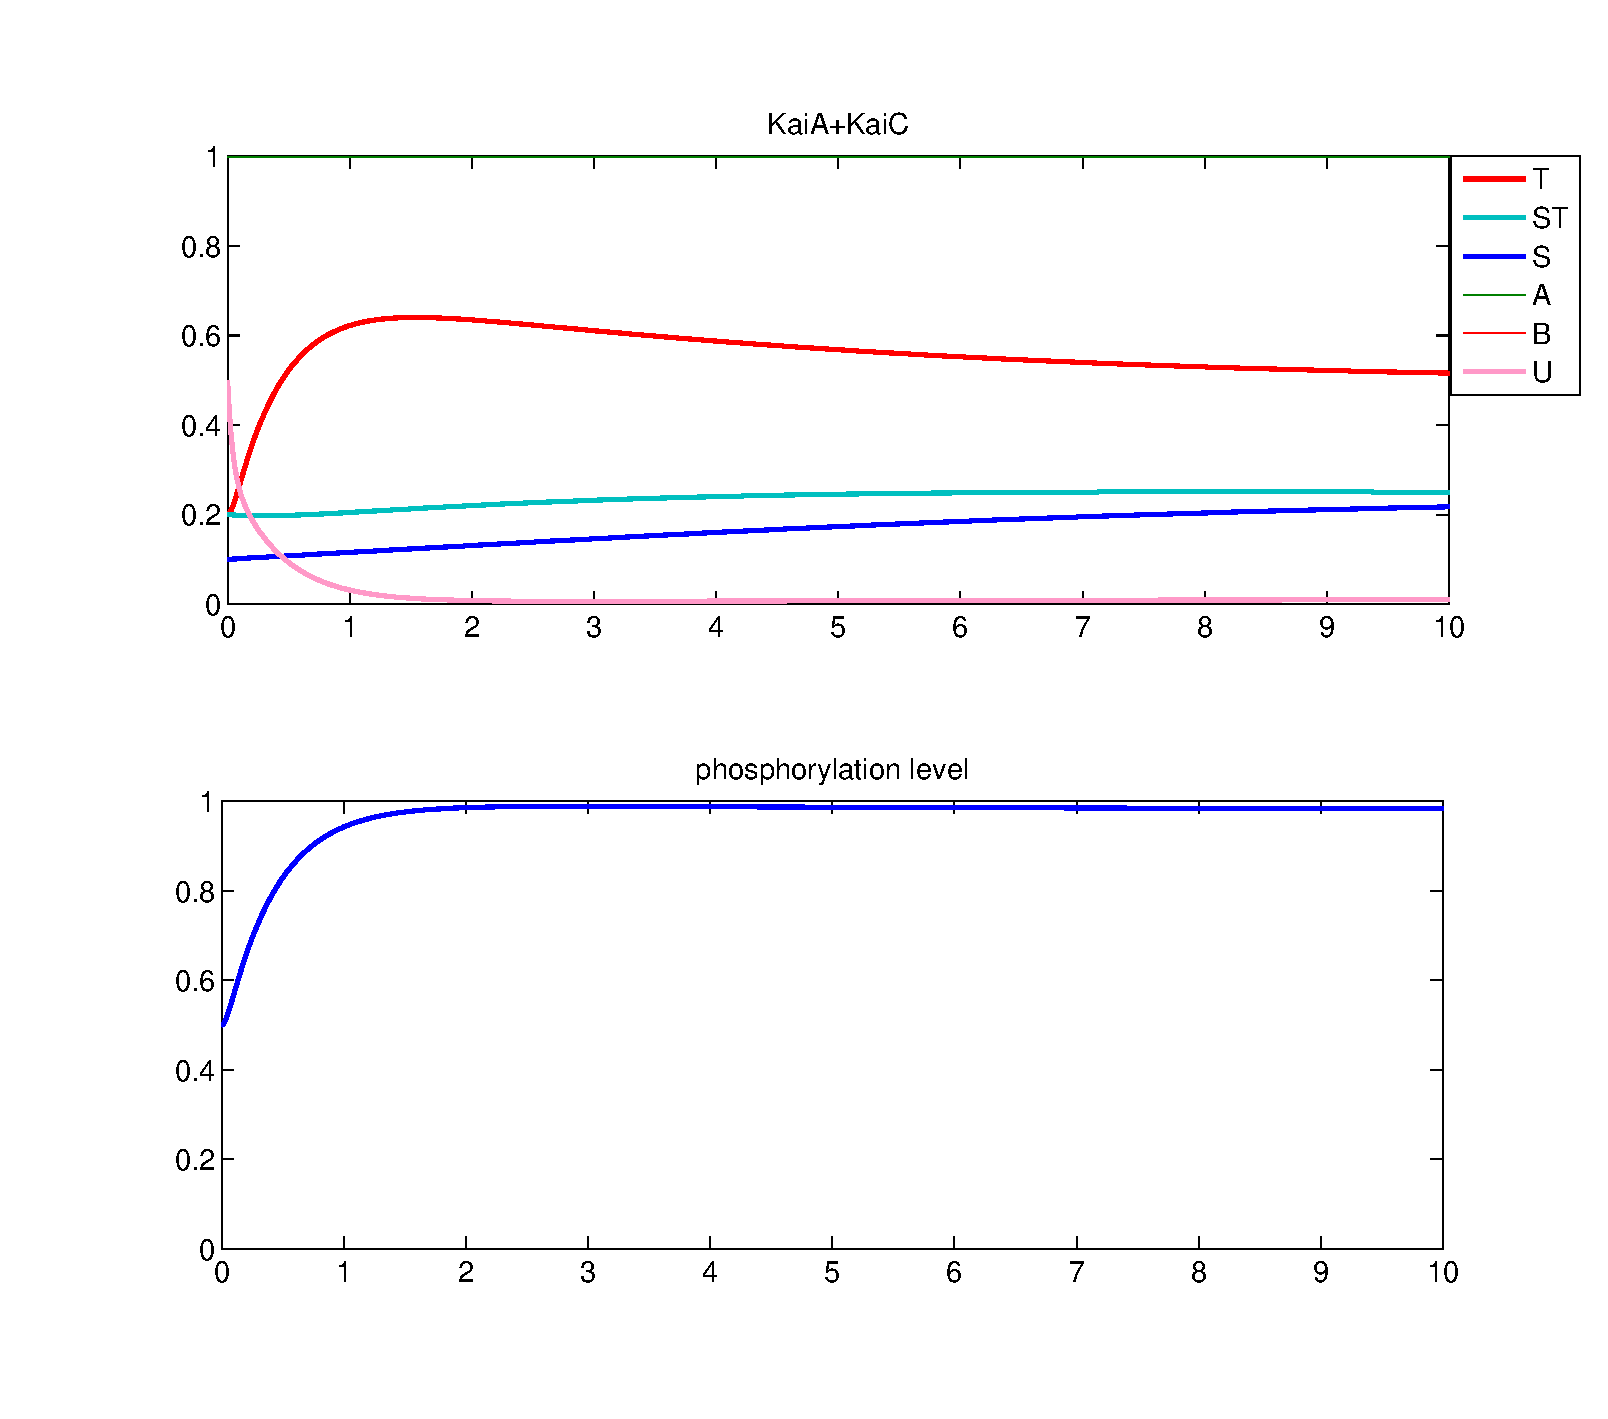
\includegraphics[scale=0.6]{A+C.eps}
\caption{\fontfamily{lmss}\selectfont Temporal profiles of different KaiC complexes as well as the overall phosphorylation level when KaiC is incubated with KaiA. The phosphorylation level reaches nearly 100\% within a short period of time. Initially KaiC is 50\% phosphorylated. Complexes that remain zero concentration due to initial conditions are omitted in the graph.}
\label{fig:A+C}
\end{figure}
\section{Temperature Compensation}
An important feature of circadian clocks, which is also true for most biological clocks, is their ability to remain at an almost unchanged period while environmental temperature can vary. This feature is known as 'temperature compensation', meaning that the effect of changes in temperature is compensated through an endogenous mechanism controlling the clock. A natural question to ask then is how this temperature-compensation is realized in circadian clocks, enabling robust regulations of biological behaviors essential to organisms.


Mathematical analysis (SI) shows that if all reactions respond to temperature changes in the same way, increasing temperature is equivalent to speeding up the time process. Therefore biological circadian clocks can not maintain a 24-h period at various temperature unless the reactions respond to temperature changes in a non-homogeneous way.

Different theories have been proposed to explain the mechanism behind temperature compensation, yet it still remains an active research area. \citet{hastings1957} propose a theory that certain reactions in a system is more sensitive to temperatures than others and some reactions can serve as temperature compensation elements, meaning that the effect of all reactions are balanced overall. \citet{lakin1991} also points out the possibility of increased amplitude while temperature increases, which serves as the counterpart of increased reaction rates. 


It is known that most reactions happen when two molecules collide with enough energy (sometimes called activation energy) and when they are head in some appropriate direction. We also know from statistical mechanics that most reaction rates follows the Arrhenius relation $k=A\exp(-E/RT)$, where $E$ is the activation energy, $R$ is the gas constant and $T$ is the absolute temperature. In other words, most reaction rates strongly depend on temperature.

In a biological system, we consider all reactions $R_i$'s and the corresponding rate constants $k_i$'s, indexed by $i$. Then the reaction rates depend on temperature following the Arrhenius relation $k_i=A_i\; e^{-E_i/RT}$.

Suppose the differential equations describing the dynamics of the system are: 
\begin{equation}\label{eq:original}
\frac{d X_j}{dt} = f_j(\overrightarrow{X})  \quad j=1,2,...,N
\end{equation} 
where $X_j$'s are the state variables and each $f_j$ is a linear combination of terms in the form $k_iX_1^{a_1}X_2^{a_2}\cdots X_N^{a_N}$ following the law of mass action. 
If all reactions speed up at the same rate when the temperature increases, can the system be temperature-compensated? To answer this question, we assume that all $k_i$'s are increased by the same factor $p$, then the right hand side of each equation is also multiplied by a factor $p$ since the new linear combination term becomes $p*k_iX_1^{a_1}X_2^{a_2}\cdots X_N^{a_N}$:
\[
\frac{d X_j}{dt} = p*f_j(\overrightarrow{X})  \quad j=1,2,...,N 
\]
After a change of variable/scaling of time $\tilde{t}=p*t$, we can recover the system into the same form as Eq.\ref{eq:original}.
\begin{equation}
 \frac{d X_j}{d\tilde{t}} = f_j(\overrightarrow{X})  \quad j=1,2,...,N 
\end{equation}

The linear theory has been developed mathematically in many papers by Peter Ruoff and was summarized in a recent book chapter \citet{ruoff2004}. He assumed that the period $\tau$  of a biological clock can be written as a complicated yet differentiable function of all reaction rates:
\begin{equation}
\tau=F(k_1,k_2,\cdots ,k_M)
\end{equation}

Denoting temperature by $T$ again, the rate of change of period length with respect to temperature can then be computed using chain rule from  basic calculus:
\begin{equation}
\begin{split}\label{eq:rateofchange}
\frac{\partial \tau}{\partial T} &= \sum_i \frac{\partial F(k_1,k_2,\cdots ,k_M)}{\partial k_i} \frac{\partial k_i}{\partial T}\\
&=\sum_i \frac{\partial F(k_1,k_2,\cdots ,k_M)}{\partial k_i} A_i\;e^{-E_i/RT}(\frac{E_i}{RT^2})\\
&=\sum_i \frac{\partial F(k_1,k_2,\cdots ,k_M)}{\partial k_i} k_i (\frac{E_i}{RT^2})\\
&=\sum_i \frac{\partial F(k_1,k_2,\cdots ,k_M)}{\partial \ln k_i}  (\frac{E_i}{RT^2})
\end{split}
\end{equation}
where in the second line, $\frac{\partial k_i}{\partial T}$ is computed according to the Arrhenius relation $k_i=A_i\; e^{-E_i/RT}$.

Multiplying $\frac{1}{\tau}$ on both sides of the last equation in Eq.\ref{eq:rateofchange} and abbreviating $F(k_1,k_2,\cdots ,k_M)$ as $F$ we have:
\begin{equation*}
\frac{\partial \tau}{\partial T}\frac{1}{\tau}= \sum_i \frac{\partial F}{\partial \ln k_i} \frac{1}{F}  \frac{E_i}{RT^2}, 
\end{equation*}
which can be rewritten as
\begin{equation}\label{eq:integral}
\frac{\partial \ln \tau}{\partial T}= \sum_i \frac{\partial \ln F}{\partial \ln k_i} \frac{E_i}{RT^2}. 
\end{equation}

Since $\tau\neq 0$, we have
\[ \frac{\partial \tau}{\partial T} =0 \iff \frac{\partial \ln \tau}{\partial T}=0 \iff \sum_i \frac{\partial \ln F}{\partial \ln k_i} \frac{E_i}{RT^2}=0. \forall T\] 
Multiplying $RT^2$ on both sides of the equation and we obtain the  condition for temperature compensation:

\begin{equation}\label{eq:balance}
\sum_i \frac{\partial \ln  F}{\partial \ln k_i} E_i = 0
\end{equation}

Now we define the sensitivity of period to each reaction as below:
\[ \beta_i=\frac{\partial \ln  F}{\partial \ln k_i}\]

At a given temperature, we have $\beta_i>0$  for reactions that contribute positively to the period length and $\beta_i< 0$ otherwise. Temperature compensation is then realized through a weighted balance among all the sensitivity coefficients $\beta_i$'s. Therefore the Ruoff's theory is indeed  a more rigorous mathematical extension from \citet{hastings1957}. 

Under linear assumption by Ruoff, $\beta_i$'s are constants. Therefore we can integrate Eq.\ref{eq:integral} to obtain a relationship between $\tau$ and $T$:
\begin{equation}
\begin{split}
\int d\ln \tau&=\sum_i \beta_i E_i \int \frac{dT}{RT^2}\\
\ln \tau &= -\frac{1}{RT}\sum_i \beta_i E_i +C\\
\tau &= \tau_0 \exp\left({-\frac{\sum_i \beta_i E_i}{RT}}\right)
\end{split}
\end{equation}

Ruoff argues that by choosing $E_i$'s properly, the balance condition Eq.\ref{eq:balance}   can be achieved and  this  tuning is realized through evolution. In practice, one can also find potential temperature compensation elements (reactions satisfying $\frac{\partial \ln  F}{\partial \ln k_i}>0$) by investigating how the the period changes when each reaction rate is increased. Once such elements are identified, temperature compensation can be realized in the system by tuning the factors by which reaction rates speed up when temperature increases (equivalent to tuning $E_i$'s).

% We find that varying KaiB binding rates almost doesn't affect the period at all (Fig.\ref{fig:varyb}), possibly since these reactions are already fast enough and the period depend rather weakly on these rates. 

\begin{figure}[H]
\centering
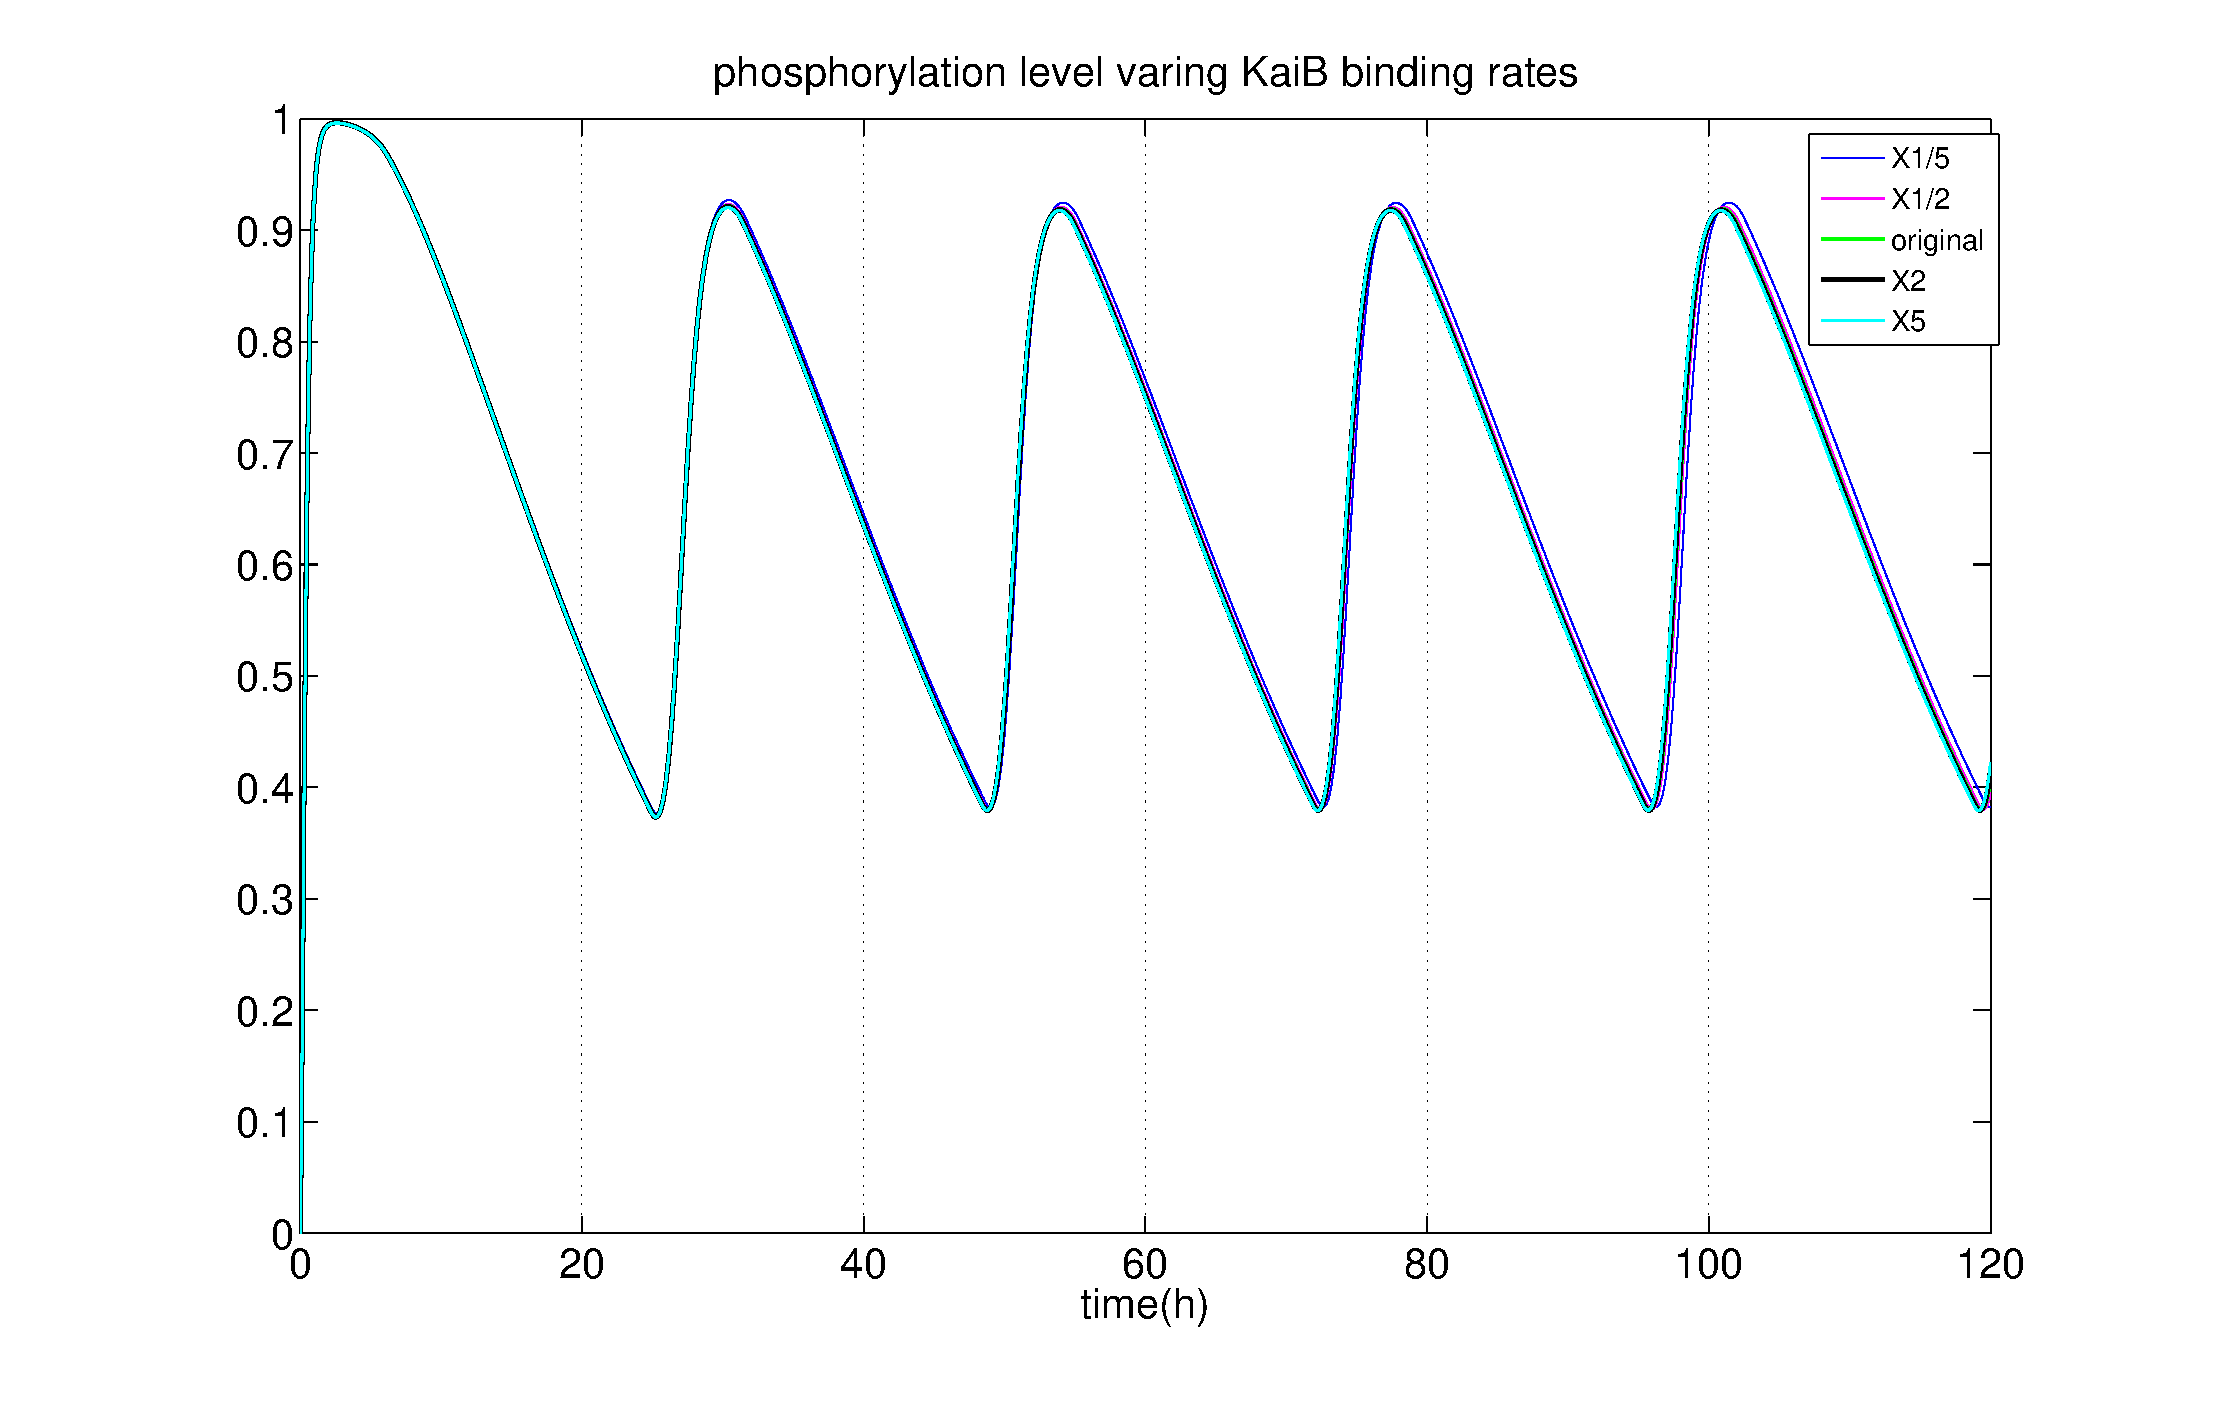
\includegraphics[scale=0.45]{tempcomp1.eps}
\caption{\fontfamily{lmss}\selectfont When KaiB binding rates are varied, the period is almost unchanged and ranges from 23.4h to 23.7h.}\label{fig:varyb}
\end{figure}

% On the other hand, KaiA binding rates are much slower, which can have a more significant effect on the period. Our simulation on varying KaiA binding rates, however, still shows rather robust period keeping with less than 10\% change (Fig.\ref{fig:varya}). Moreover, we observe some interesting phase shift which can reflect a mechanism to adjust to sudden temperature change. 




\begin{figure}[H]
\centering
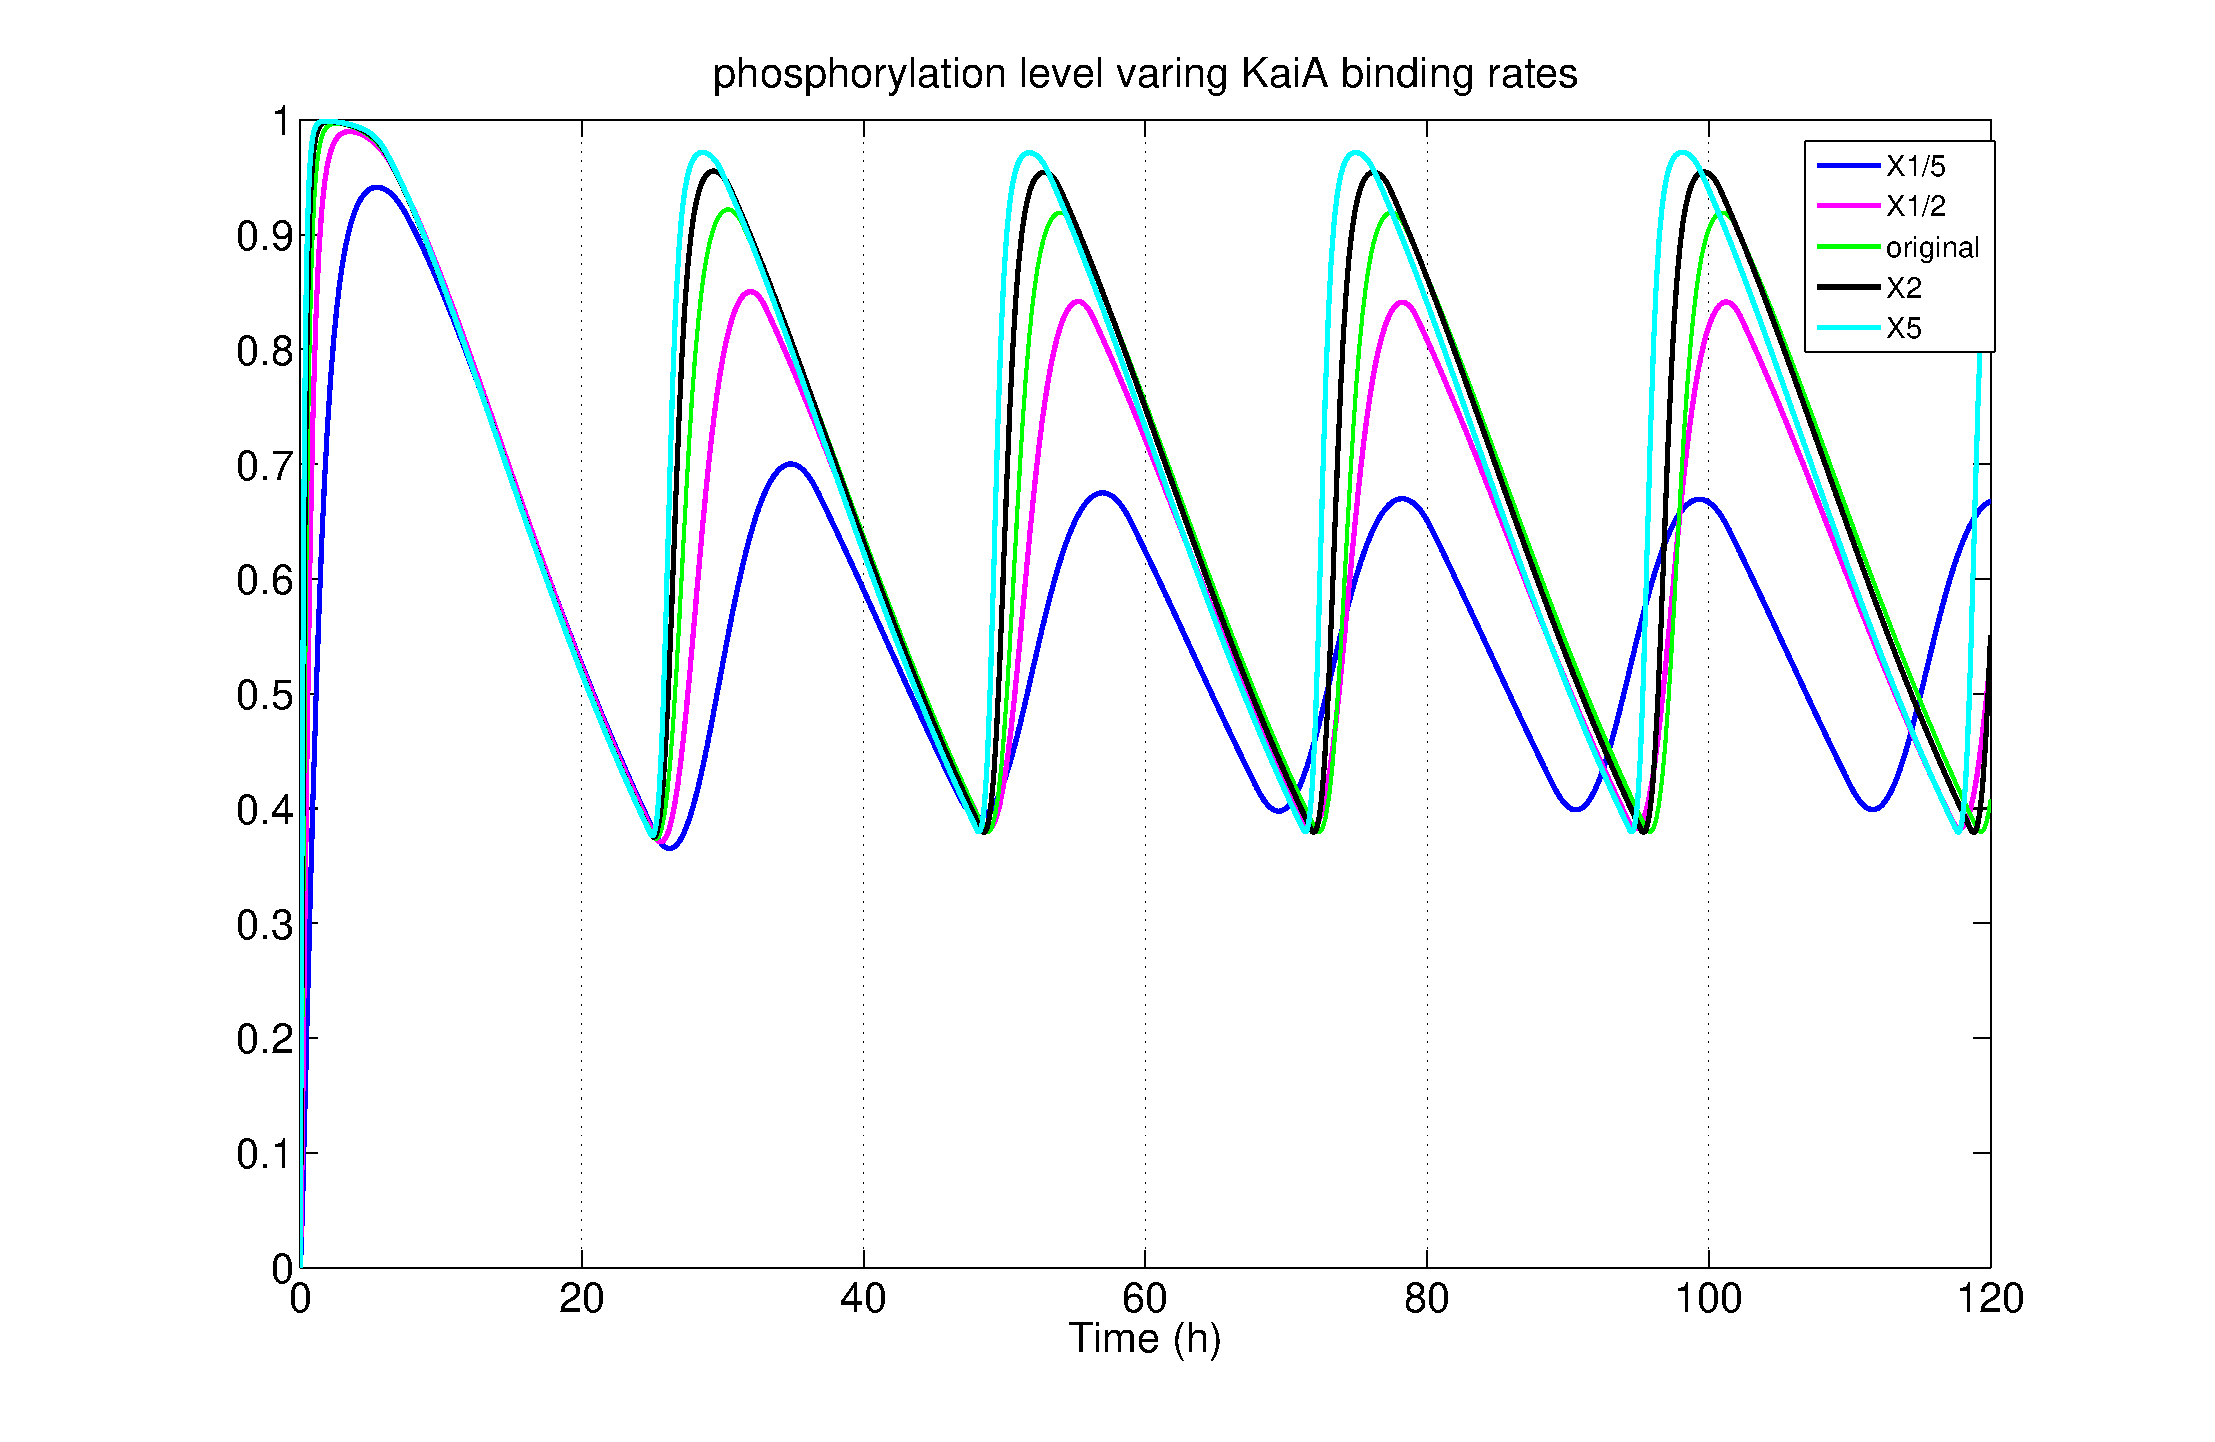
\includegraphics[scale=0.45]{tempcomp2.eps}
\caption{\fontfamily{lmss}\selectfont Period change is within 10\% (21.08h to 23.56h) and phase shift can be observed.}\label{fig:varya}
\end{figure}
% Due to the phase shift effect, period seems to change more than it actually does. Therefore we also measure the period of each case and plot it against the varying rates (Fig.\ref{fig:temcompelmt}). Surprisingly, we find that KaiA binding can in fact serve as a temperature compensation element. As described in Hastings and Sweeney's theory, slowing these rates by a factor 1/2 or 1/5 actually shortens the period. 

\begin{figure}[H]
\centering
\includegraphics[scale=0.4]{tempcomp6.eps}
\caption{\fontfamily{lmss}\selectfont Period is optimized at a roughly 24h length. Lowering the rates by a factor 1/2 or 1/5 results in a shorter period.}\label{fig:temcompelmt}
\end{figure}
% In fact, we can explain this mechanism with theory from Lakin-Thomas et al. since the amplitude of the oscillation is increased when the reaction rates are increased (Fig.\ref{fig:ampvary}). 

\begin{figure}[H]
\centering
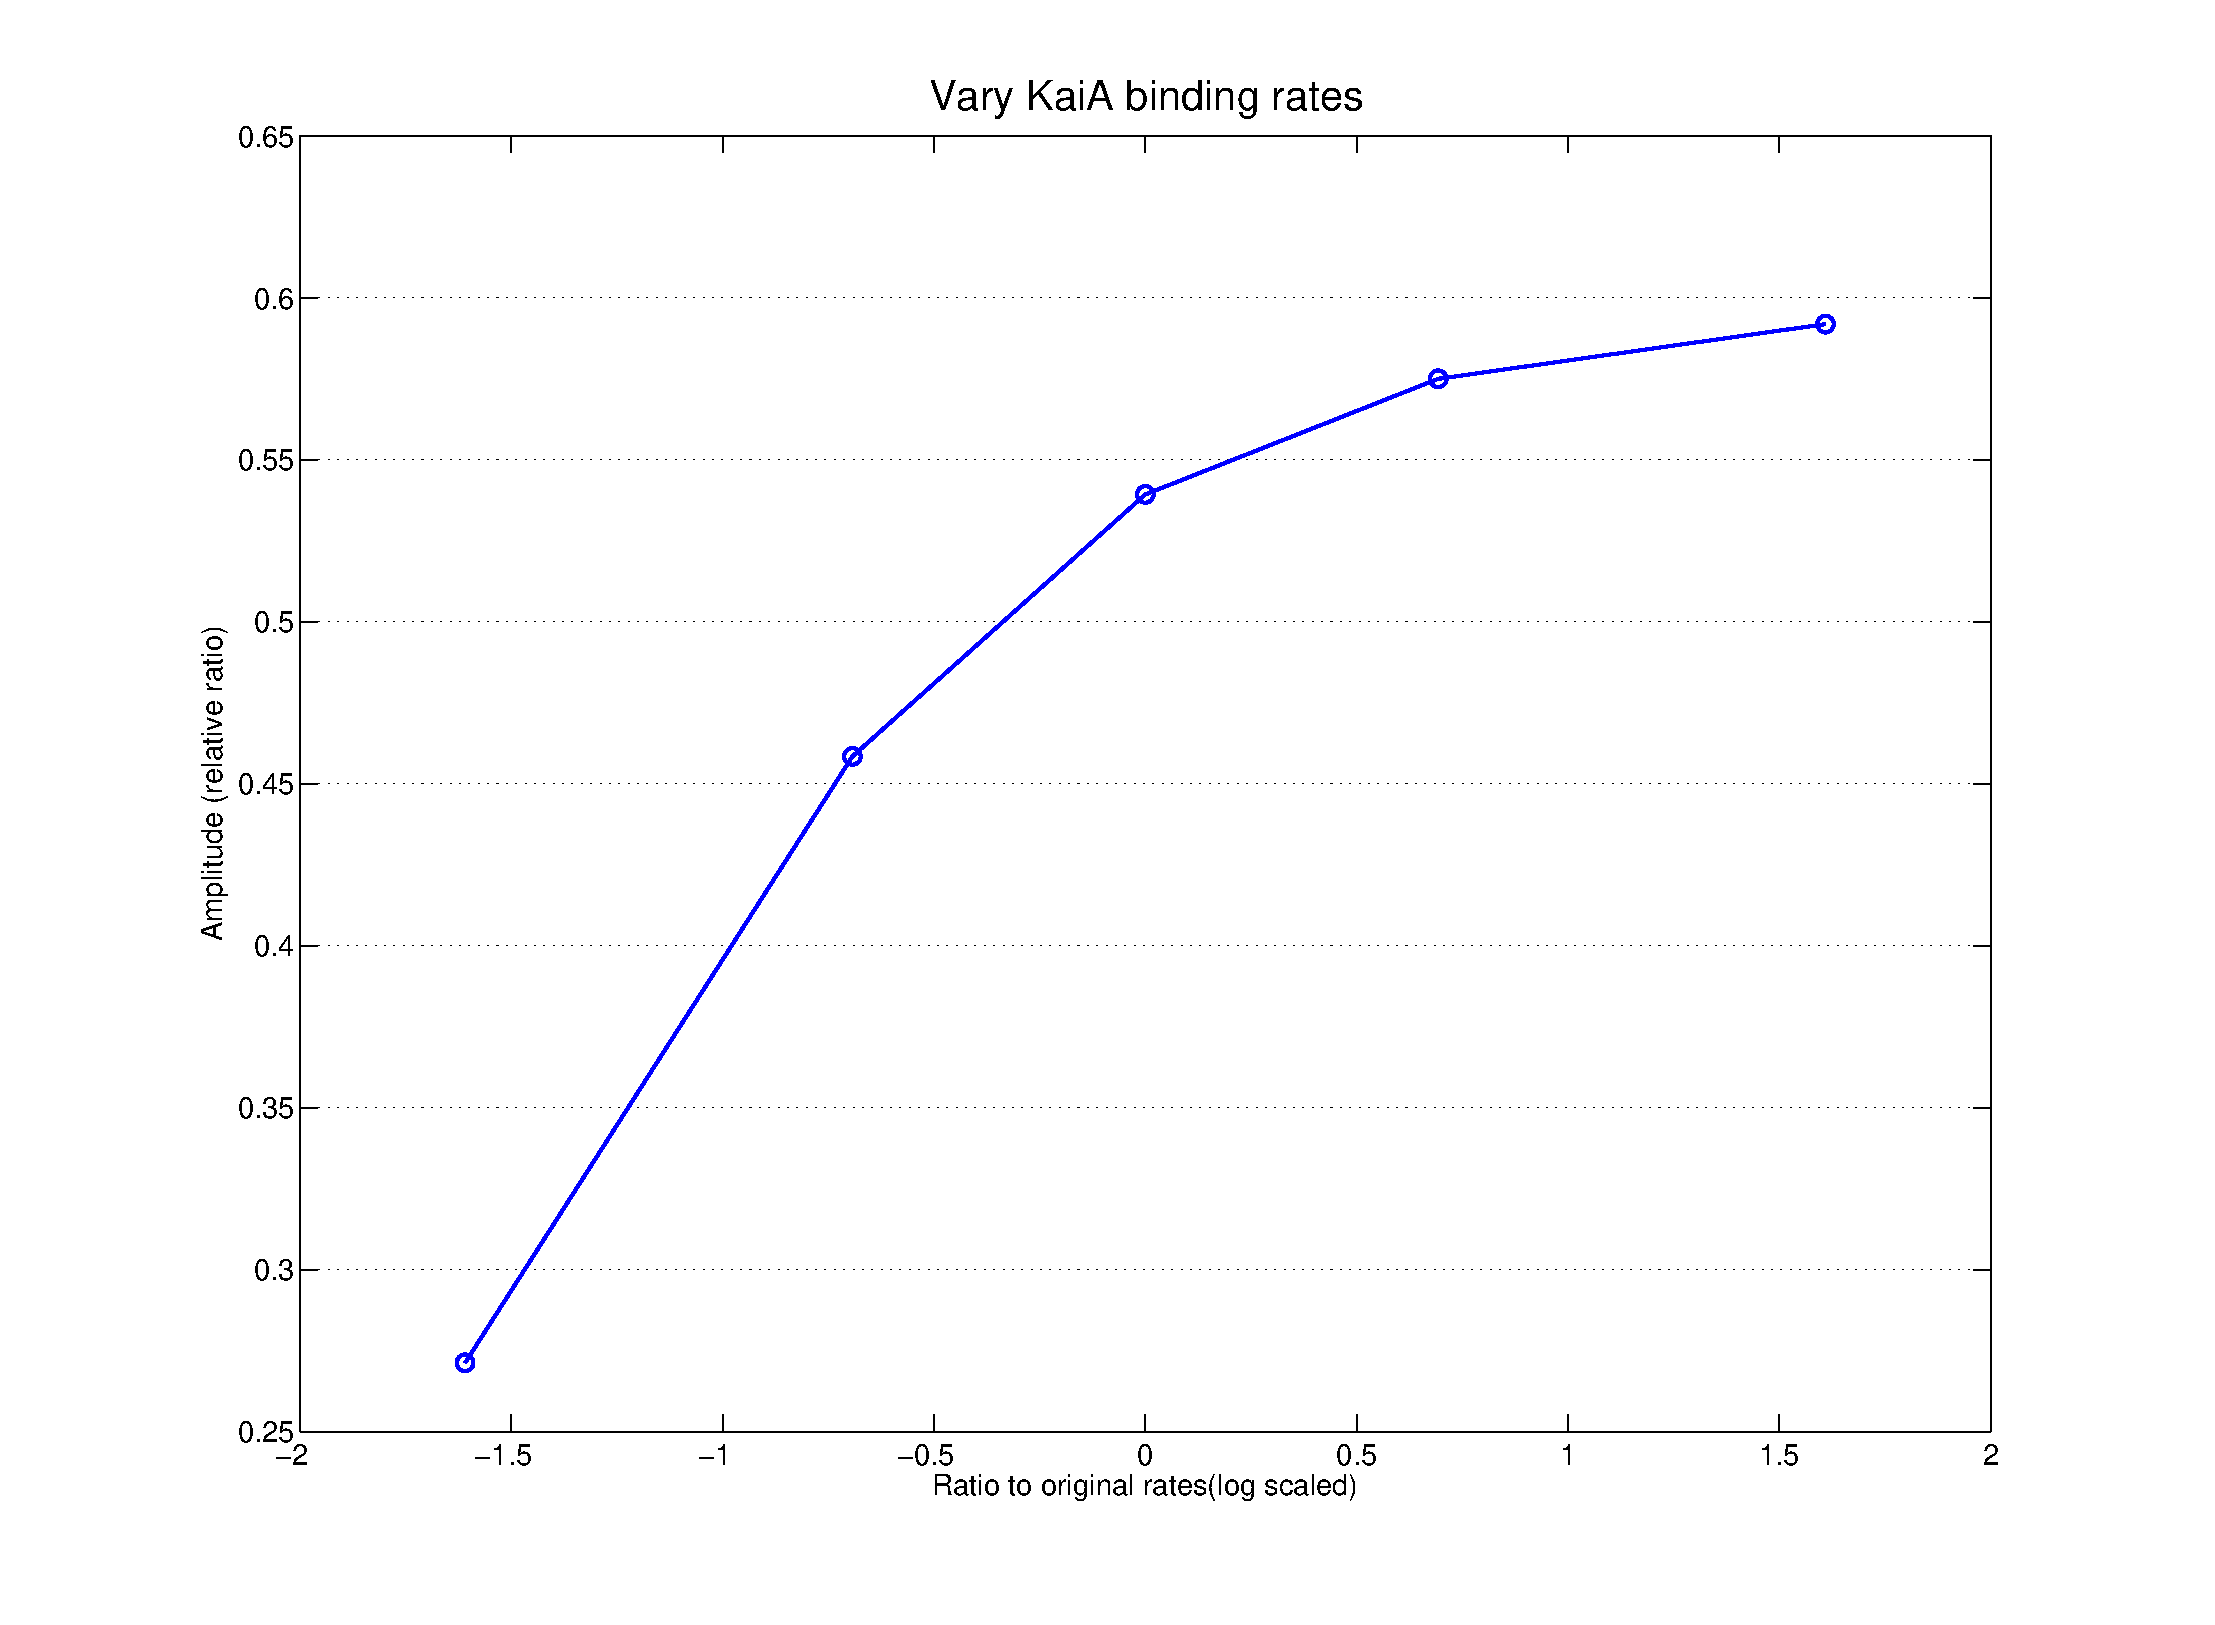
\includegraphics[scale=0.4]{tempcomp7.eps}
\caption{\fontfamily{lmss}\selectfont Amplitude increases as the reaction rates increases.}\label{fig:ampvary}
\end{figure}

% We therefore conclude that the KaiA-activated autokinase reaction can also serve as a temperature compensation element since when temperature is decreased, period is shortened while amplitude is decreased (Fig.\ref{fig:varycat} and Fig. \ref{fig:tempcomp8}). 

\begin{figure}[H]
\centering
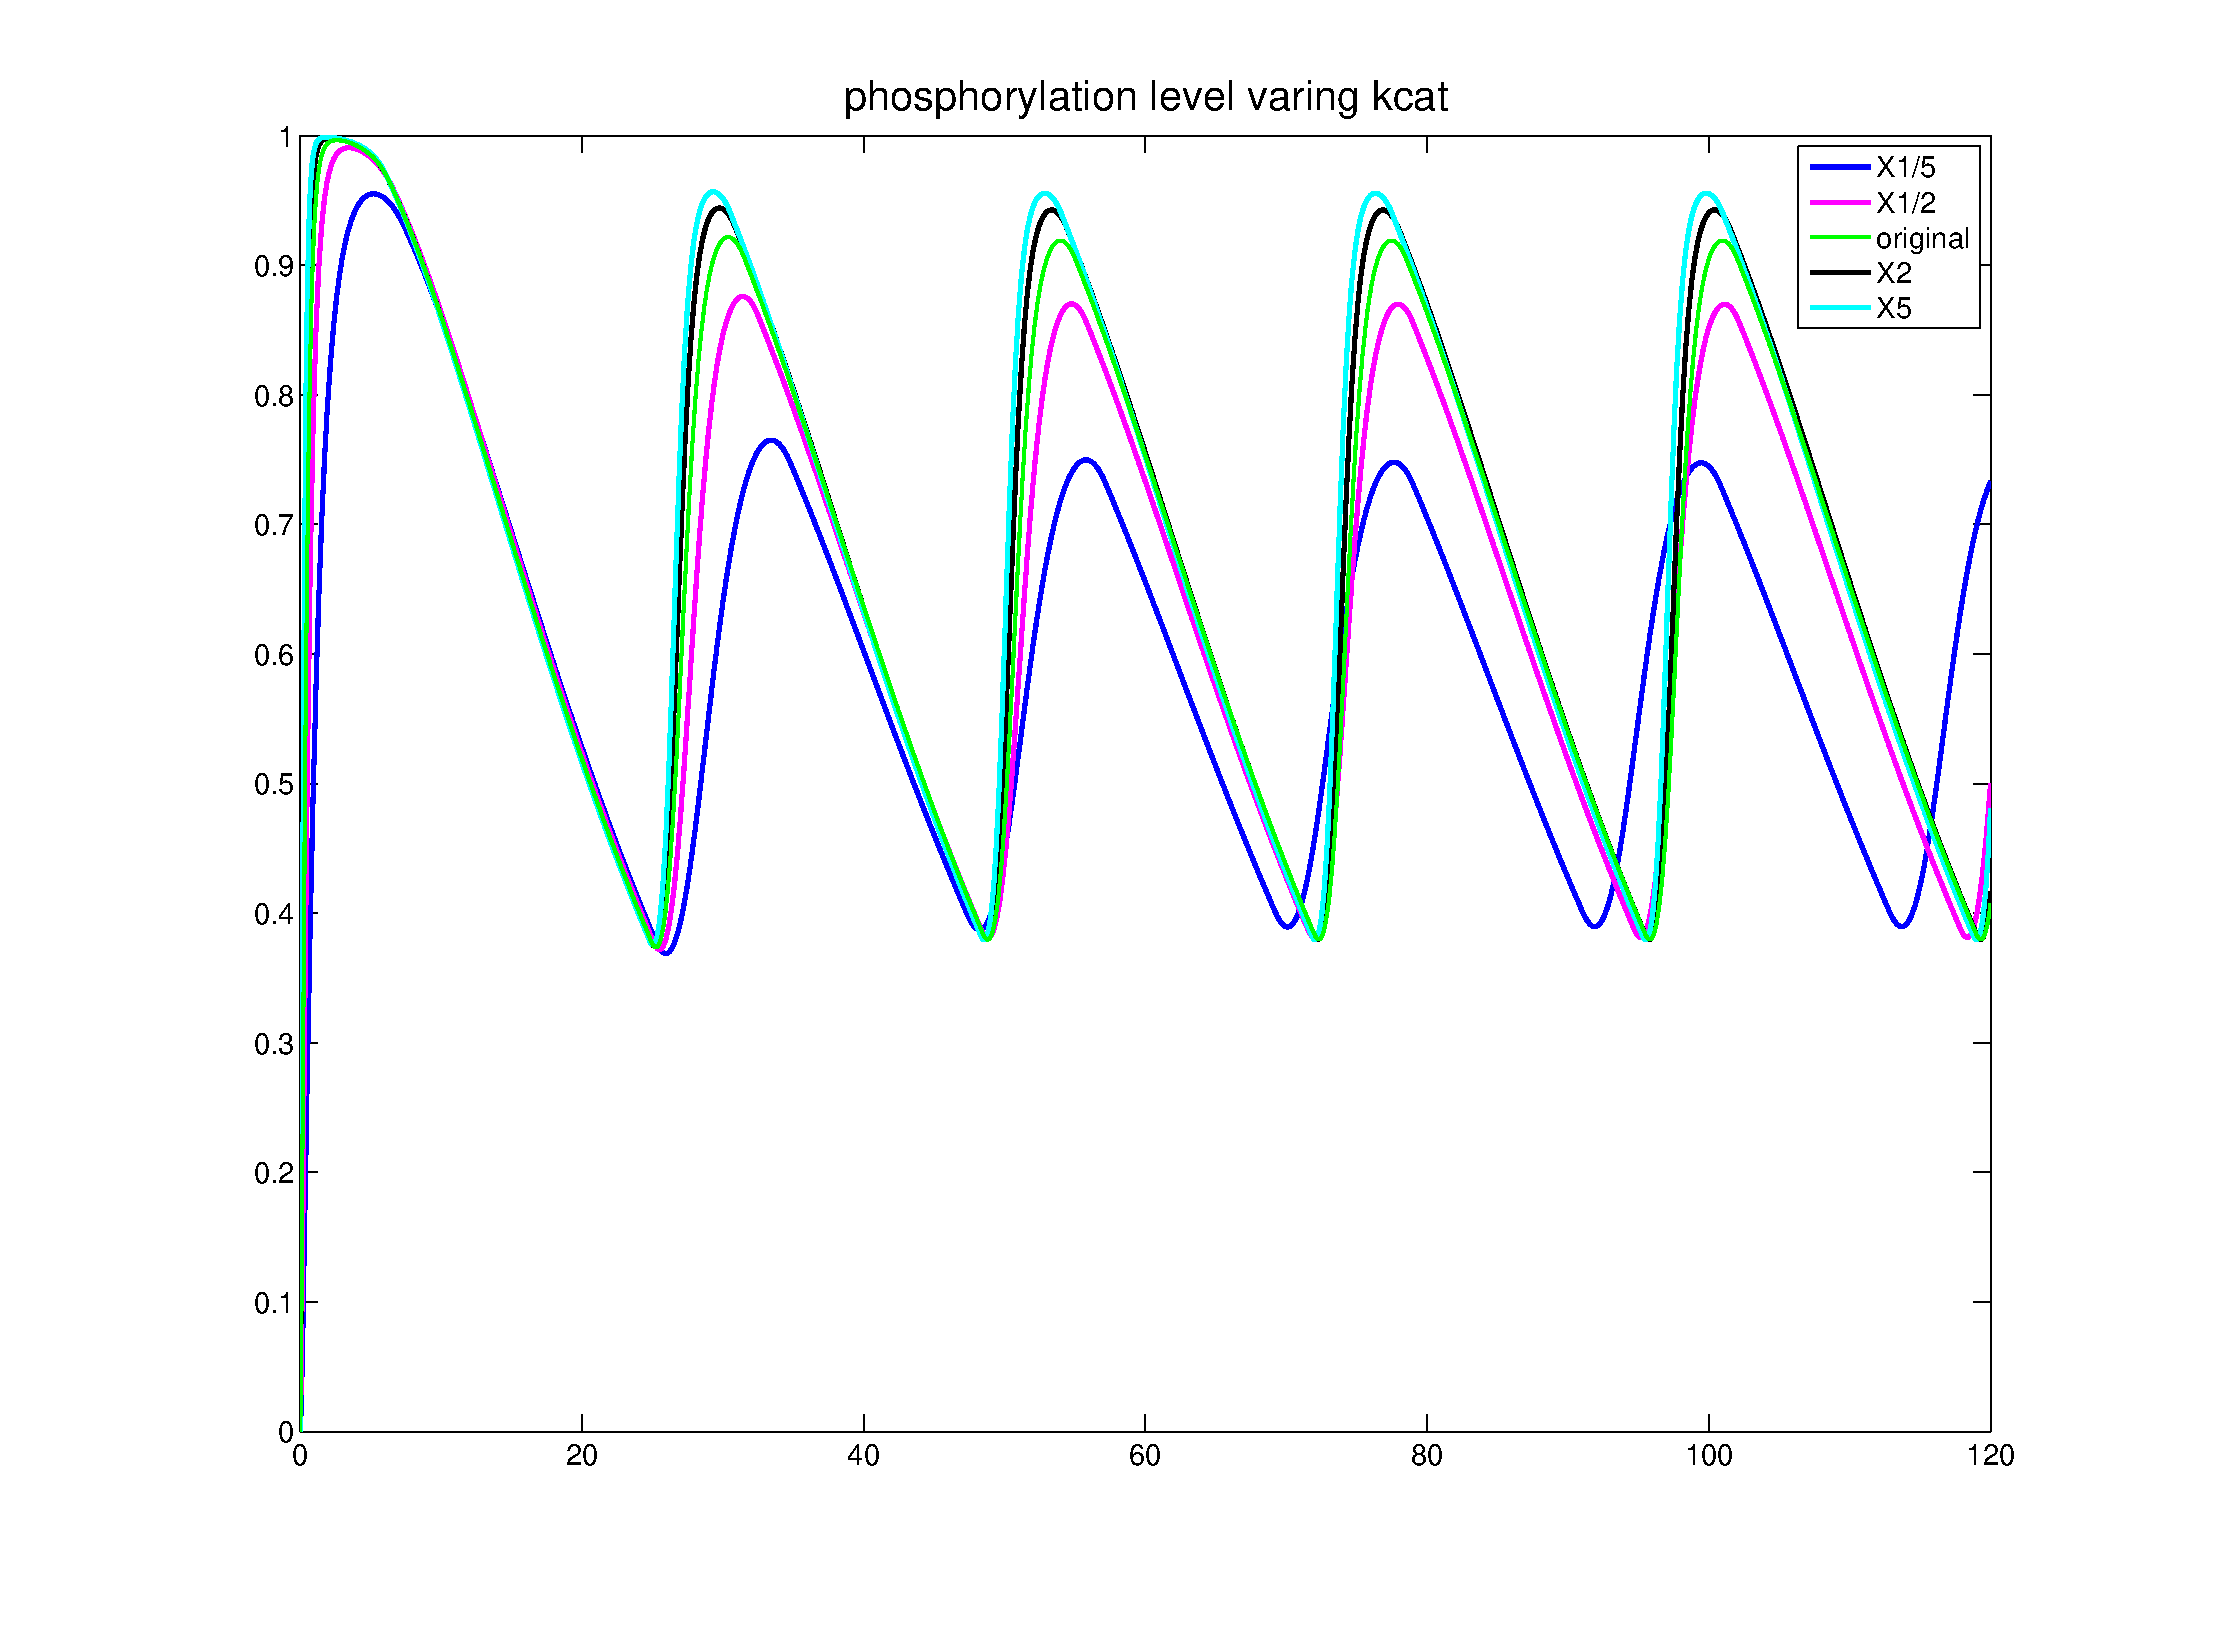
\includegraphics[scale=0.4]{tempcomp5.eps}
\caption{\fontfamily{lmss}\selectfont Different time profiles while varying KaiA-activated autokinase reaction rates.}
\label{fig:varycat}
\end{figure}

\begin{figure}[H]
\centering
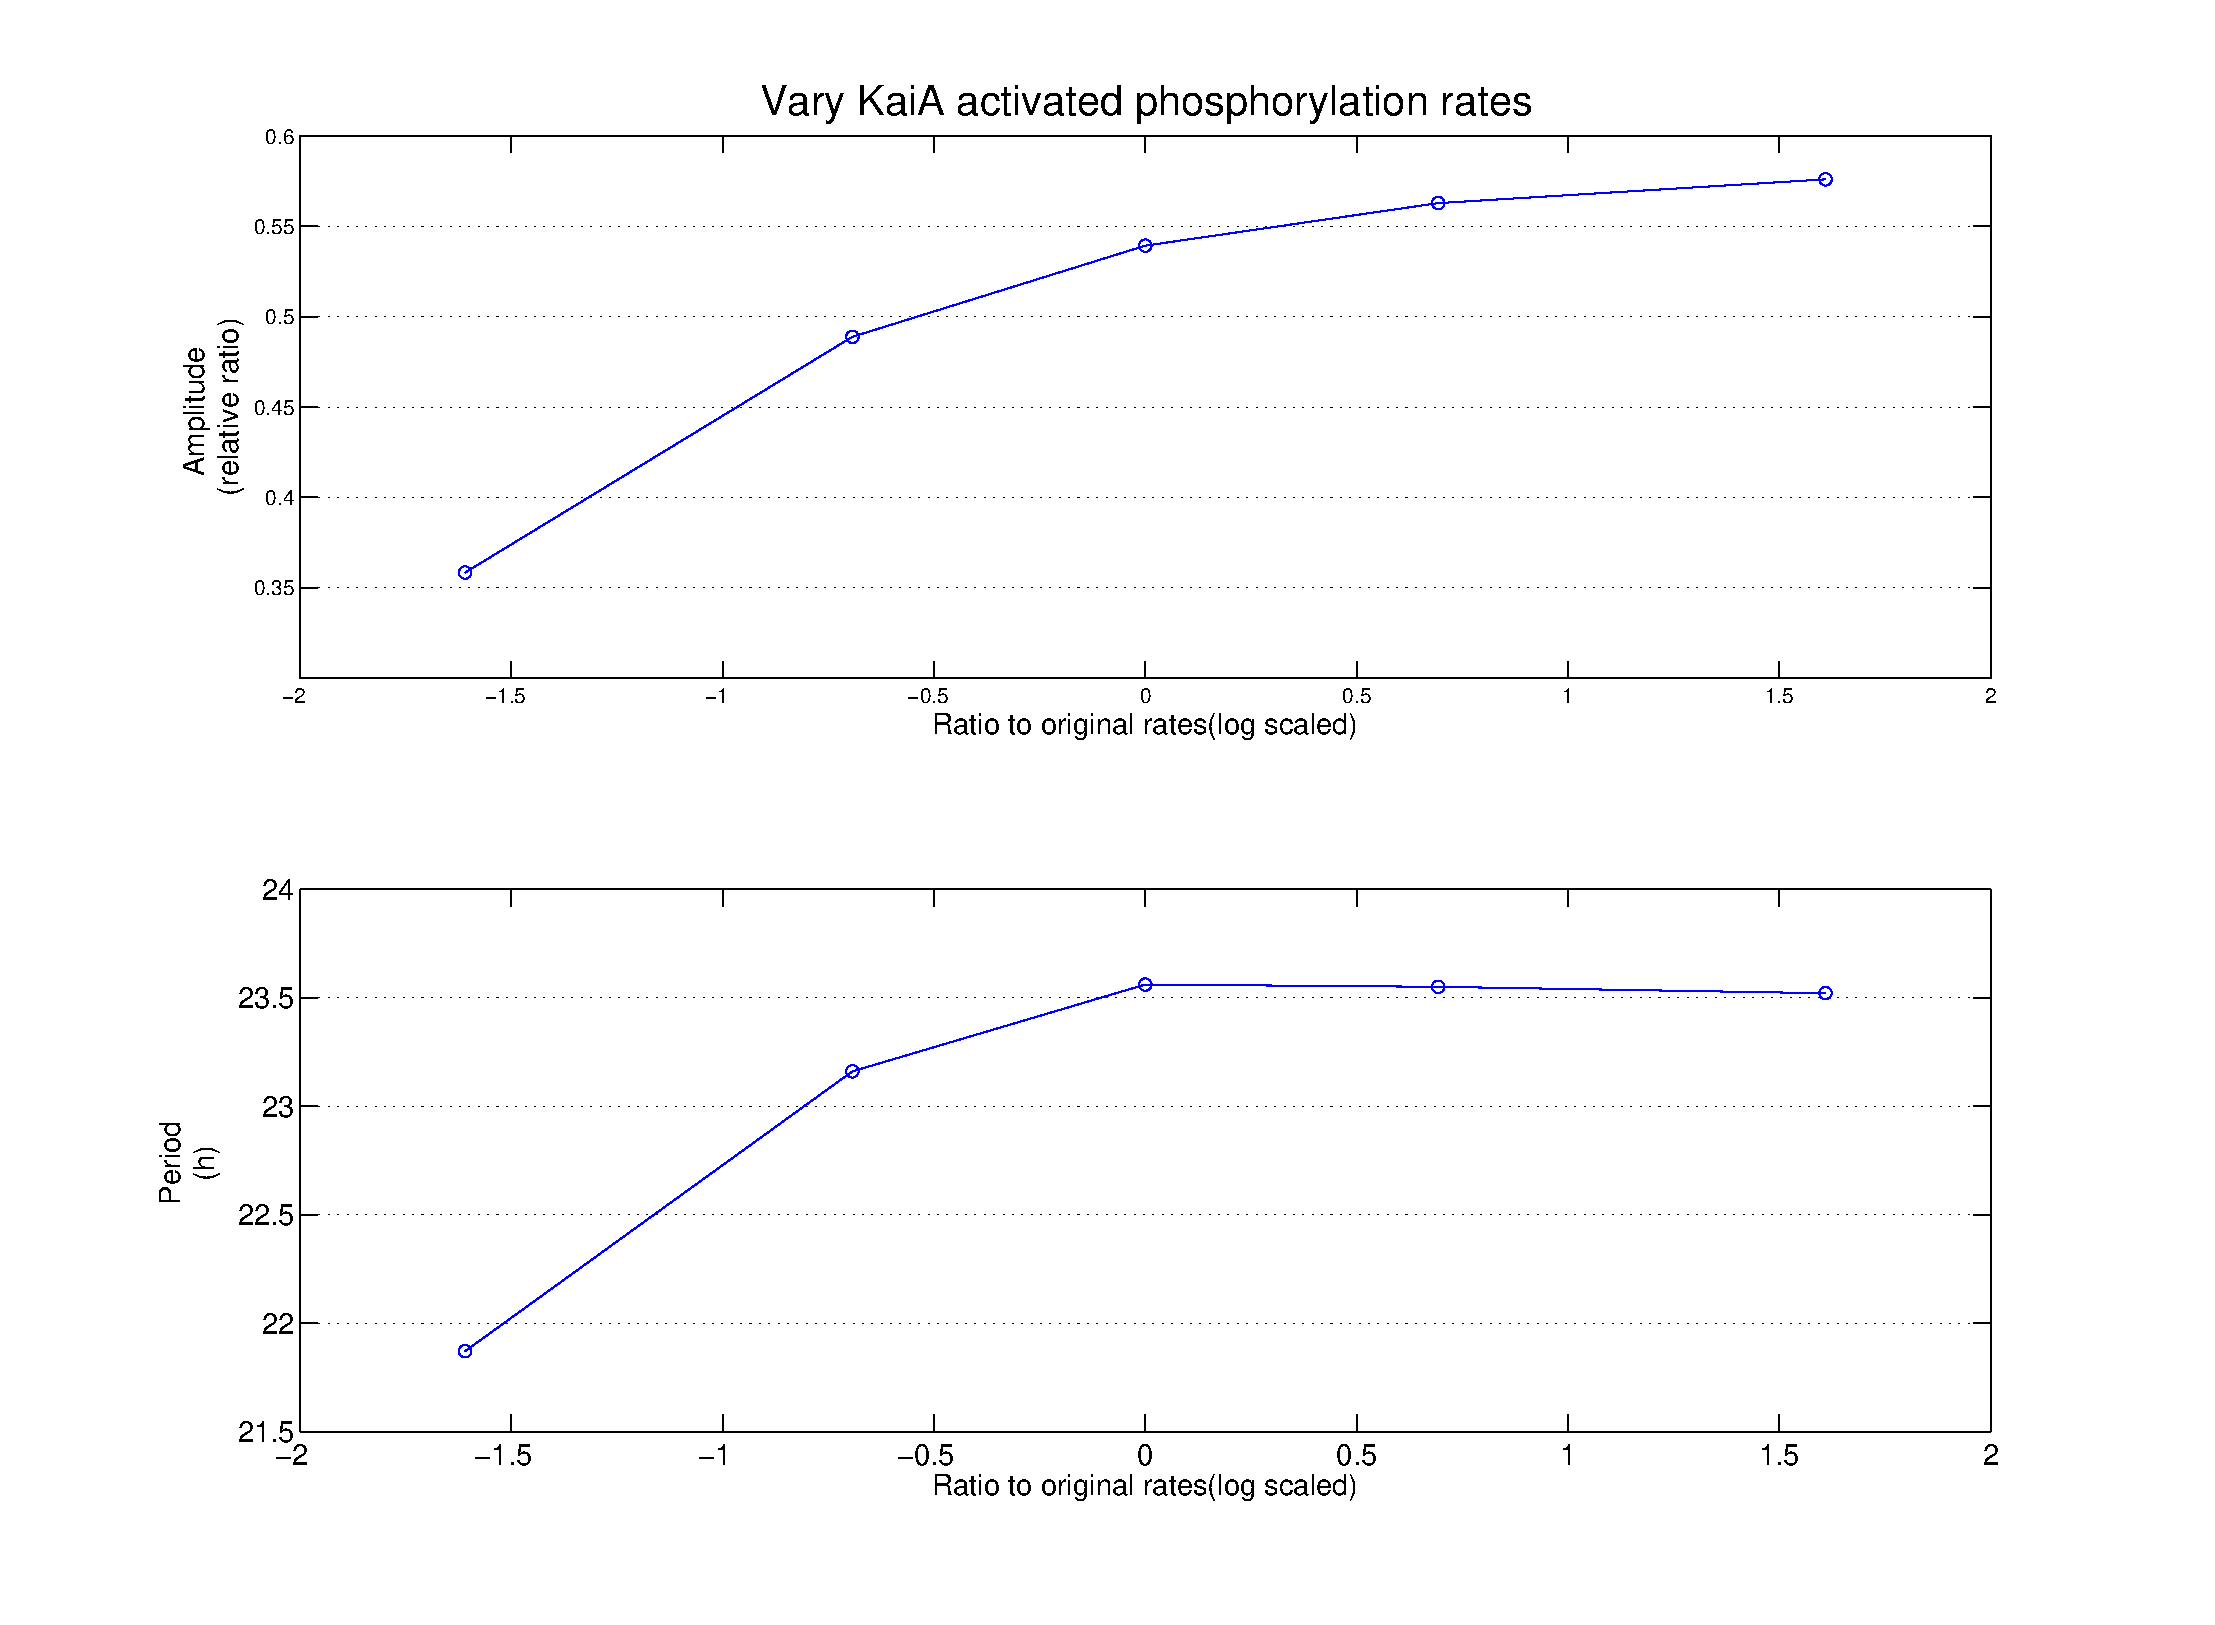
\includegraphics[scale=0.4]{tempcomp8.eps}
\caption{\fontfamily{lmss}\selectfont Period is optimized at a roughly 24h length. Lowering the rates by a factor 1/2 or 1/5 results in a shorter period. Amplitude increases as the reaction rates increases.}\label{fig:tempcomp8}
\end{figure}
\bibliography{review}
\end{document}